\documentclass[11pt]{article}
%%%%%%%%% options for the file macros.tex

\def\showauthornotes{1}
\def\showkeys{0}
\def\showdraftbox{0}
% \allowdisplaybreaks[1]

%% Shamelessly adapted from a scribe template by Sanjeev Arora

%%%%%%%%%%%%%% Packages
% \usepackage[active,tightpage]{preview}
% \renewcommand{\PreviewBorder}{1in}
\usepackage[hidelinks]{hyperref}
\usepackage{amsmath,amssymb,amsthm,amstext,amsfonts,bbm,algorithm,algorithmicx,xspace,nicefrac,
  algpseudocode}
\usepackage{color,stmaryrd,enumerate,latexsym,bm,amsfonts,
  subfigure,wrapfig,verbatim,tabularx,textcomp}
\usepackage[small]{caption}
\usepackage{comment} 
\usepackage{epsfig} 
\usepackage{latexsym,nicefrac,bbm}
\usepackage{xspace}
\usepackage{color,fancybox,graphicx,url,subfigure}
\usepackage{enumitem, fullpage}
\usepackage{booktabs}
\usepackage{commath}
\usepackage{mdframed}
\usepackage{pdfsync}
\usepackage{tikz}
\usetikzlibrary {positioning}

%%%%%%%%%%%%%% Use for definitions
\newcommand{\defeq}{\stackrel{\textup{def}}{=}}

\DeclareMathOperator*{\argmax}{arg\,max}
\DeclareMathOperator*{\argmin}{arg\,min}

%%%%%%%%%%%%%% Theorem Environments
\newtheorem{theorem}{Theorem}[section]
\newtheorem{problem}[theorem]{Problem}
\newtheorem{lemma}[theorem]{Lemma}
\newtheorem{definition}[theorem]{Definition}
\newtheorem{corollary}[theorem]{Corollary}
\newtheorem{conjecture}[theorem]{Conjecture}
\newtheorem{proposition}[theorem]{Proposition}
\newtheorem{fact}[theorem]{Fact}
\newtheorem{remark}[theorem]{Remark}

%%%%%%%%%%%%%% Probability stuff
\DeclareMathOperator*{\pr}{\bf Pr}
\DeclareMathOperator*{\av}{\mathbbm{E}}
\DeclareMathOperator*{\var}{\bf Var}

%%%%%%%%%%%%%% Matrix stuff
\newcommand{\tr}[1]{\mathop{\mbox{Tr}}\left({#1}\right)}
\newcommand{\diag}[1]{{\bf Diag}\left({#1}\right)}

%% Notation for integers, natural numbers, reals, fractions, sets, cardinalities
%%and so on
\newcommand{\nfrac}[2]{\nicefrac{#1}{#2}}
\def\abs#1{\left| #1 \right|}
\renewcommand{\norm}[1]{\ensuremath{\left\lVert #1 \right\rVert}}

\newcommand{\floor}[1]{\left\lfloor\, {#1}\,\right\rfloor}
\newcommand{\ceil}[1]{\left\lceil\, {#1}\,\right\rceil}

\newcommand{\pair}[1]{\left\langle{#1}\right\rangle} %for inner product

\newcommand\B{\{0,1\}}      % boolean alphabet  use in math mode
\newcommand\bz{\mathbb Z}
\newcommand\nat{\mathbb N}
\newcommand\rea{\mathbb R}
\newcommand\com{\mathbb{C}}
\newcommand\plusminus{\{\pm 1\}}
\newcommand\Bs{\{0,1\}^*}   % B star use in math mode
\newcommand{\ones}{\mathbbm{1}}
\newcommand{\eye}{\mathbbm{I}}



\newcommand{\V}[1]{\mathbf{#1}\ignorespaces}
\renewcommand\AA{\boldsymbol{\mathit{A}}}
\newcommand\LL{\boldsymbol{\mathit{L}}}

% Used to denote bold commands
                                % e.g. vectors, matrices
\DeclareRobustCommand{\fracp}[2]{{#1 \overwithdelims()#2}}
\DeclareRobustCommand{\fracb}[2]{{#1 \overwithdelims[]#2}}
\newcommand{\marginlabel}[1]%
{\mbox{}\marginpar{\it{\raggedleft\hspace{0pt}#1}}}
\newcommand\card[1]{\left| #1 \right|} %cardinality of set S; usage \card{S}
\renewcommand\set[1]{\left\{#1\right\}} %usage \set{1,2,3,,}
\renewcommand\complement{\ensuremath{\mathsf{c}}}
\newcommand\poly{\mbox{poly}}  %usage \poly(n)
\newcommand{\comp}[1]{\overline{#1}}
\newcommand{\smallpair}[1]{\langle{#1}\rangle}
\newcommand{\ol}[1]{\ensuremath{\overline{#1}}\xspace}
\newcommand{\eps}{\epsilon}
\DeclareMathOperator{\vol}{\mathsf{vol}}


%%%%%%%%%%%%%% Mathcal shortcuts
\newcommand\calF{\mathcal{F}}
\newcommand\calP{\mathcal{P}}
\newcommand\calS{\mathcal{S}}
\newcommand\calG{\mathcal{G}}
\newcommand\calH{\mathcal{H}}
\newcommand\calC{\mathcal{C}}
\newcommand\calD{\mathcal{D}}
\newcommand\calI{\mathcal{I}}
\newcommand\calV{\mathcal{V}}
\newcommand\calK{\mathcal{K}}
\newcommand\calN{\mathcal{N}}
\newcommand\calX{\mathcal{X}}
\newcommand\calU{\mathcal{U}}
\newcommand\calE{\mathcal{E}}
\newcommand\calL{\mathcal{L}}
\newcommand\calR{\mathcal{R}}


%%%%%%%%%%%%%% {{{ authornotes }}}
\definecolor{Mygray}{gray}{0.8}

 \ifcsname ifcommentflag\endcsname\else
  \expandafter\let\csname ifcommentflag\expandafter\endcsname
                  \csname iffalse\endcsname
\fi

\ifnum\showauthornotes=1
\newcommand{\todo}[1]{\colorbox{Mygray}{\color{red}#1}}
\else
\newcommand{\todo}[1]{#1}
\fi

\ifnum\showauthornotes=1
\newcommand{\Authornote}[2]{{\sf\small\color{red}{[#1: #2]}}}
\newcommand{\Authoredit}[2]{{\sf\small\color{red}{[#1]}\color{blue}{#2}}}
\newcommand{\Authorcomment}[2]{{\sf \small\color{gray}{[#1: #2]}}}
\newcommand{\Authorfnote}[2]{\footnote{\color{red}{#1: #2}}}
\newcommand{\Authorfixme}[1]{\Authornote{#1}{\textbf{??}}}
\newcommand{\Authormarginmark}[1]{\marginpar{\textcolor{red}{\fbox{%\Large
#1:!}}}}
\else
\newcommand{\Authornote}[2]{}
\newcommand{\Authoredit}[2]{}
\newcommand{\Authorcomment}[2]{}
\newcommand{\Authorfnote}[2]{}
\newcommand{\Authorfixme}[1]{}
\newcommand{\Authormarginmark}[1]{}
\fi


%%%%%%%%%%%%%% Logical operators
\newcommand\true{\mbox{\sc True}}
\newcommand\false{\mbox{\sc False}}
\def\scand{\mbox{\sc and}}
\def\scor{\mbox{\sc or}}
\def\scnot{\mbox{\sc not}}
\def\scyes{\mbox{\sc yes}}
\def\scno{\mbox{\sc no}}

%% Parantheses
\newcommand{\paren}[1]{\unskip\left({#1}\right)}
\newcommand{\sqparen}[1]{\unskip\left[{#1}\right]}
\newcommand{\curlyparen}[1]{\unskip\left\{{#1}\right\}}
\newcommand{\smallparen}[1]{\unskip({#1})}
\newcommand{\smallsqparen}[1]{\unskip[{#1}]}
\newcommand{\smallcurlyparen}[1]{\unskip\{{#1}\}}

%% short-hands for relational simbols

\newcommand{\from}{:}
\newcommand\xor{\oplus}
\newcommand\bigxor{\bigoplus}
\newcommand{\logred}{\leq_{\log}}
\def\iff{\Leftrightarrow}
\def\implies{\Rightarrow}

%--------------------------------------------------------------------------------------------------------------------------------
% Optimization macros
%--------------------------------------------------------------------------------------------------------------------------------
%\providecommand{\argmax}{\mathop\mathrm{arg max}} % Defining math symbols
%\providecommand{\argmin}{\mathop\mathrm{arg min}}
\providecommand{\arccos}{\mathop\mathrm{arccos}}
\providecommand{\dom}{\mathop\mathrm{dom}}
\providecommand{\diag}{\mathop\mathrm{diag}}
\providecommand{\tr}{\mathop\mathrm{tr}}
%\providecommand{\abs}{\mathop\mathrm{abs}}
\providecommand{\card}{\mathop\mathrm{card}}
\providecommand{\sign}{\mathop\mathrm{sign}}
\providecommand{\conv}{\mathop\mathrm{conv}} % Convex hull
\def\rank#1{\mathrm{rank}({#1})}
\def\supp#1{\mathrm{supp}({#1})}

\providecommand{\minimize}{\mathop\mathrm{minimize}}
\providecommand{\maximize}{\mathop\mathrm{maximize}}
\providecommand{\subjectto}{\mathop\mathrm{subject\;to}}

%\renewcommand\eqref[1]{Eq.~(\ref{#1})}

\def\openright#1#2{\left[{#1}, {#2}\right)}

%--------------------------------------------------------------------------------------------------------------------------------
% Vectors and matrices
%--------------------------------------------------------------------------------------------------------------------------------
\newcommand{\boldone}{\mbf{1}} % Bold 1
\newcommand{\ident}{\mbf{I}} % Identity matrix
% \def\v#1{\mbi{#1}} % Vector notation
%\def\norm#1{\left\|{#1}\right\|} % A norm with 1 argument
\newcommand{\onenorm}[1]{\norm{#1}_1} % L1 norm
\newcommand{\twonorm}[1]{\norm{#1}_2} % L2 norm
\newcommand{\infnorm}[1]{\norm{#1}_{\infty}} % Linfty norm
\newcommand{\opnorm}[1]{\norm{#1}_{\text{op}}} % Operator norm
\newcommand{\fronorm}[1]{\norm{#1}_{\text{F}}} % Frobenius norm
\newcommand{\nucnorm}[1]{\norm{#1}_{*}} % Frobenius norm
\def\staticnorm#1{\|{#1}\|} % A static norm that does not resize with input
\newcommand{\statictwonorm}[1]{\staticnorm{#1}_2} % L2 norm
\newcommand{\inner}[1]{{\langle #1 \rangle}} % inner product
\newcommand{\binner}[2]{\left\langle{#1},{#2}\right\rangle} % Inner product with expandable brackets
\def\what#1{\widehat{#1}}

\def\twovec#1#2{\left[\begin{array}{c}{#1} \\ {#2}\end{array}\right]}
\def\threevec#1#2#3{\left[\begin{array}{c}{#1} \\ {#2} \\ {#3} \end{array}\right]}
\def\nvec#1#2#3{\left[\begin{array}{c}{#1} \\ {#2} \\ \vdots \\ {#3}\end{array}\right]} % An n-vector with three arguments
\DeclareMathOperator\spn{span}


%% macros to write pseudo-code

\newlength{\pgmtab}  %  \pgmtab is the width of each tab in the
\setlength{\pgmtab}{1em}  %  program environment
 \newenvironment{program}{\renewcommand{\baselinestretch}{1}%
\begin{tabbing}\hspace{0em}\=\hspace{0em}\=%
\hspace{\pgmtab}\=\hspace{\pgmtab}\=\hspace{\pgmtab}\=\hspace{\pgmtab}\=%
\hspace{\pgmtab}\=\hspace{\pgmtab}\=\hspace{\pgmtab}\=\hspace{\pgmtab}\=%
\+\+\kill}{\end{tabbing}\renewcommand{\baselinestretch}{\intl}}
\newcommand {\BEGIN}{{\bf begin\ }}
\newcommand {\ELSE}{{\bf else\ }}
\newcommand {\IF}{{\bf if\ }}
\newcommand {\FOR}{{\bf for\ }}
\newcommand {\TO}{{\bf to\ }}
\newcommand {\DO}{{\bf do\ }}
\newcommand {\WHILE}{{\bf while\ }}
\newcommand {\ACCEPT}{{\bf accept}}
\newcommand {\REJECT}{\mbox{\bf reject}}
\newcommand {\THEN}{\mbox{\bf then\ }}
\newcommand {\END}{{\bf end}}
\newcommand {\RETURN}{\mbox{\bf return\ }}
\newcommand {\HALT}{\mbox{\bf halt}}
\newcommand {\REPEAT}{\mbox{\bf repeat\ }}
\newcommand {\UNTIL}{\mbox{\bf until\ }}
\newcommand {\TRUE}{\mbox{\bf true\ }}
\newcommand {\FALSE}{\mbox{\bf false\ }}
\newcommand {\FORALL}{\mbox{\bf for all\ }}
\newcommand {\DOWNTO}{\mbox{\bf down to\ }}

% Theorem-type environments
% \theoremstyle{break} 
% \theoremheaderfont{\scshape}
% \theorembodyfont{\slshape}
% \newtheorem{Thm}{Theorem}[section]
% \newtheorem{Lem}[Thm]{Lemma}
% \newtheorem{Cor}[Thm]{Corollary}
% \newtheorem{Prop}[Thm]{Proposition}
% % \theoremstyle{plain} 
% % \theorembodyfont{\rmfamily} 
% \newtheorem{Ex}[Thm]{Exercise}
% \newtheorem{Exa}[Thm]{Example}
% \newtheorem{Rem}[Thm]{Remark}
% % \theorembodyfont{\itshape}
% \newtheorem{Def}[Thm]{Definition}
% \newtheorem{Conj}[Thm]{Conjecture}
% \newtheorem{Obs}[Thm]{Observation}
% \newtheorem{Ques}[Thm]{Question}
%\newenvironment{proof}{\noindent {\sc Proof:}}{$\Box$ \medskip} 
\newenvironment{problems} % Definition of problems
 {\renewcommand{\labelenumi}{\S\theenumi}
	\begin{enumerate}}{\end{enumerate}}


%%%%%%%%%%%%%%%%% Proof Environments

\def\FullBox{\hbox{\vrule width 6pt height 6pt depth 0pt}}
%
%\def\qed{\ifmmode\qquad\FullBox\else{\unskip\nobreak\hfil
%\penalty50\hskip1em\null\nobreak\hfil\FullBox
%\parfillskip=0pt\finalhyphendemerits=0\endgraf}\fi}

\def\qedsketch{\ifmmode\Box\else{\unskip\nobreak\hfil
\penalty50\hskip1em\null\nobreak\hfil$\Box$
\parfillskip=0pt\finalhyphendemerits=0\endgraf}\fi}

%\newenvironment{proof}{\begin{trivlist} \item {\bf Proof:~~}}
 %  {\qed\end{trivlist}}

\newenvironment{proofsketch}{\begin{trivlist} \item {\bf
Proof Sketch:~~}}
  {\qedsketch\end{trivlist}}

\newenvironment{proofof}[1]{\begin{trivlist} \item {\bf Proof
#1:~~}}
  {\qed\end{trivlist}}

\newenvironment{claimproof}{\begin{quotation} \noindent
{\bf Proof of claim:~~}}{\qedsketch\end{quotation}}


%%%%%%%%%%%%%%%%%%%%%%%%%%%%%%%%%%%%%%%%%%%%%%%%%%%%%%%%%%%%%%%%%%%%%%%%%%%
%%%%%%%%%%%%%%%%%%%%%%%%%%%%%%%%%%%%%%%%%%%%%%%%%%%%%%%%%%%%%%%%%%%%%%%%%%%




\newlength{\tpush}
\setlength{\tpush}{2\headheight}
\addtolength{\tpush}{\headsep}

\newcommand{\handout}[5]{
   \noindent
   \begin{center}
   \framebox{ \vbox{ \hbox to \textwidth { {\bf \coursenum\ :\  \coursename} \hfill #5 }
       \vspace{3mm}
       \hbox to \textwidth { {\Large \hfill #2  \hfill} }
       \vspace{1mm}
       \hbox to \textwidth { {\it #3 \hfill #4} }
     }
   }
   \end{center}
   \vspace*{4mm}
   \newcommand{\lecturenum}{#1}
   \addcontentsline{toc}{chapter}{Lecture #1 -- #2}
}

\newcommand{\lecturetitle}[4]{\handout{#1}{#2}{Lecturer: \courseprof
  }{Scribes: #3}{Date: #4}}
\newcommand{\guestlecturetitle}[5]{\handout{#1}{#2}{Lecturer:
    #4}{Scribe: #3}{Lecture #1 - #5}}


%%%%%%%%%%%%%%%%%%%%%%%%%%%%%%%%%%%%%%%%%%%%%%%%%%%%%%%%%
%%% Commands to include figures


%% PSfigure

\newcommand{\PSfigure}[3]{\begin{figure}[t] 
  \centerline{\vbox to #2 {\vfil \psfig{figure=#1.eps,height=#2} }} 
  \caption{#3}\label{#1} 
  \end{figure}} 
\newcommand{\twoPSfigures}[5]{\begin{figure*}[t]
  \centerline{%
    \hfil
    \begin{tabular}{c}
        \vbox to #3 {\vfil\psfig{figure=#1.eps,height=#3}} \\ (a)
    \end{tabular}
    \hfil\hfil\hfil
    \begin{tabular}{c}
        \vbox to #3 {\vfil\psfig{figure=#2.eps,height=#3}} \\ (b)
    \end{tabular}
    \hfil}
  \caption{#4}
  \label{#5}
%  \sublabel{#1}{(a)}
%  \sublabel{#2}{(b)}
  \end{figure*}}

\newcounter{fignum}

% fig
%command to insert figure. usage \fig{name}{h}{caption}
%where name.eps is the postscript file and h is the height in inches
%The figure is can be referred to using \ref{name}
\newcommand{\fig}[3]{%
\begin{minipage}{\textwidth}
\centering\epsfig{file=#1.eps,height=#2}
\caption{#3} \label{#1}
\end{minipage}
}%


% ffigure
% Usage: \ffigure{name of file}{height}{caption}{label}
\newcommand{\ffigure}[4]{\begin{figure} 
  \centerline{\vbox to #2 {\hfil \psfig{figure=#1.eps,height=#2} }} 
  \caption{#3}\label{#4} 
  \end{figure}} 

% ffigureh
% Usage: \ffigureh{name of file}{height}{caption}{label}
\newcommand{\ffigureh}[4]{\begin{figure}[!h] 
  \centerline{\vbox to #2 {\vfil \psfig{figure=#1.eps,height=#2} }} 
  \caption{#3}\label{#4} 
  \end{figure}} 


% {{{ draftbox }}}
\ifnum\showdraftbox=1
\newcommand{\draftbox}{\begin{center}
  \fbox{%
    \begin{minipage}{2in}%
      \begin{center}%
%        \begin{Large}%
          \large\textsc{Working Draft}\\%
%        \end{Large}\\
        Please do not distribute%
      \end{center}%
    \end{minipage}%
  }%
\end{center}
\vspace{0.2cm}}
\else
\newcommand{\draftbox}{}
\fi


%% Complexity classes
\newcommand\p{\mbox{\bf P}\xspace}
\newcommand\np{\mbox{\bf NP}\xspace}
\newcommand\cnp{\mbox{\bf coNP}\xspace}
\newcommand\sigmatwo{\mbox{\bf $\Sigma_2$}\xspace}
\newcommand\ppoly{\mbox{\bf $\p_{\bf /poly}$}\xspace}
\newcommand\sigmathree{\mbox{\bf $\Sigma_3$}\xspace}
\newcommand\pitwo{\mbox{\bf $\Pi_2$}\xspace}
\newcommand\rp{\mbox{\bf RP}\xspace}
\newcommand\zpp{\mbox{\bf ZPP}\xspace}
\newcommand\bpp{\mbox{\bf BPP}\xspace}
\newcommand\ph{\mbox{\bf PH}\xspace}
\newcommand\pspace{\mbox{\bf PSPACE}\xspace}
\newcommand\npspace{\mbox{\bf NPSPACE}\xspace}
\newcommand\dl{\mbox{\bf L}\xspace}
\newcommand\ma{\mbox{\bf MA}\xspace}
\newcommand\am{\mbox{\bf AM}\xspace}
\newcommand\nl{\mbox{\bf NL}\xspace}
\newcommand\conl{\mbox{\bf coNL}\xspace}
\newcommand\sharpp{\mbox{\#{\bf P}}\xspace}
\newcommand\parityp{\mbox{$\oplus$ {\bf P}}\xspace}
\newcommand\ip{\mbox{\bf IP}\xspace}
\newcommand\pcp{\mbox{\bf PCP}}
\newcommand\dtime{\mbox{\bf DTIME}}
\newcommand\ntime{\mbox{\bf NTIME}}
\newcommand\dspace{\mbox{\bf SPACE}\xspace}
\newcommand\nspace{\mbox{\bf NSPACE}\xspace}
\newcommand\cnspace{\mbox{\bf coNSPACE}\xspace}
\newcommand\exptime{\mbox{\bf EXP}\xspace}
\newcommand\nexptime{\mbox{\bf NEXP}\xspace}
\newcommand\genclass{\mbox{$\cal C$}\xspace}
\newcommand\cogenclass{\mbox{\bf co$\cal C$}\xspace}
\newcommand\size{\mbox{\bf SIZE}\xspace}
\newcommand\sig{\mathbf \Sigma}
\newcommand\pip{\mathbf \Pi}

%%Computational problems
\newcommand\sat{\mbox{SAT}\xspace}
\newcommand\tsat{\mbox{3SAT}\xspace}
\newcommand\tqbf{\mbox{TQBF}\xspace}
\allowdisplaybreaks

\usepackage{tikz, mathtools}
\usepackage[
    backend=biber,
% giveninits=true,
% natbib=true,
    style=alphabetic,
    url=false, 
 %   doi=true,
    hyperref,
    backref=true,
    backrefstyle=none,
    maxbibnames=10,
    sortcites
]{biblatex}
%\usepackage{subfigure}
% \usepackage{subcaption}
\usepackage{graphicx}
\addbibresource{ref.bib}

%%%%%%%%% Authornotes
\newcommand{\Snote}{\Authornote{S}}




%\newcommand\eqdef{\stackrel{\mathclap{\normalfont\mbox{def}}}{=}}
\newcommand\idenVec{\V{1}}
% \DeclareMathOperator{\vol}{Vol}
\newcommand\nuReq{y^\top\V{D}\V{1}=0}
\newcommand\nuFrac{\frac{y^\top\V{L}y}{y^\top\V{D}y}}


\addbibresource{refs.bib}

%%%%%%%%%%%%%%%%%%%%%%%%%

\begin{document}

\newcommand{\coursenum}{{CSC 2240H}}
\newcommand{\coursename}{{Graphs, Matrices, and Optimization}}
\newcommand{\courseprof}{Sushant Sachdeva}

\lecturetitle{1}{Generating Uniform Spanning Trees}{Haonan Duan, Yangjun Ruan}{\today}

In this lecture, we introduce two randomized algorithms for generating spanning trees uniformly. Given a connected, undirected and unweighted graph
$G(V, E)$ with $n$ vertices and $m$ edges, the goal is to generate a spanning tree $T$ of $G$ chosen \textbf{uniformly} at random among all spanning trees of $G$. Recall that a spanning tree $T$ of an undirected graph $G$ is a subgraph that is a tree which includes all vertices of $G$.

\section{The first algorithm: random walk}

A random walk on $G$ is a Markov chain over all vertices with the transition matrix:
\begin{equation*}
    P(w|v) = \begin{cases} 
      \frac{1}{r_v} & \text{if } $(v, w)$ \text{ is an edge.} \\
      0 & \text{o.w.}
   \end{cases}
\end{equation*}

where $r_v$ is the degree of the node $v$.

\begin{algorithm}
\caption*{$\textsc{Algorithm I \cite{aldous1990random} \cite{broder1989generating}}$}
\begin{algorithmic}
%\State Construct a probabililty distribution $\{p_e\}_{e\in E_G}$
%\INDENT
    \State  Simulate a simple random walk on the graph G starting at an arbitrary vertex $s$ until every vertex is visited. For each vertex $i \in V - s$ collect the edge $\{j, i\}$ that corresponds to the first entrance to vertex $i$. Let $T$ be this collection of edges. Output $T$.
%\ENDINDENT
\end{algorithmic}
\end{algorithm}
Our first algorithm is that a random walk can simulate a uniform spanning tree by selecting the first edge that enters the node. The pseudocode is shown above. The running time of Algorithm I is $O(mn)$. It's clear that $T$ is a spanning tree because it contains $|V|-1$ edges and no loops. We shall prove that it is indeed uniformly distributed. 

Before discussing the algorithm, it will be useful to introduce \emph{arborescences} defined as below:
\begin{definition}{(Arborescence)}    
    For a given $s \in G$, an arborescence $T$ \emph{rooted at $s$} is a directed spanning tree of $G$ where all vertices in $G \setminus \set{s}$ have \emph{exactly one} incoming arc.
\end{definition}

It is easy to check that there is a one-to-one correspondence between spanning trees of $G$ and arborescences rooted at $s$: given any spanning tree, there is a unique way of directing its edges to make it an arborescence rooted at $s$; conversely, given any arborescence rooted at $s$, one can obtain a spanning tree by simply disregarding the direction of the edges.
Therefore, if we get a procedure that generates arborescences, it also gives a procedure that generates spanning trees. 

Indeed, random walk simulates a chain of arborescences along the way.

\begin{definition}{(Arborescence chain).}
Let $(X_j; -\infty < j < \infty)$ be the Markov chain of a random walk on $G$. We can define a Markov chain of arborescences $(S_j; -\infty < j < \infty)$. Considering $(X_j, X_{j+1}, \cdots)$, we choose $X_j$ to be the root of $S_j$ and select the first edge entering other vertices to be in the tree. In other words, the tree $S_j$ is rooted at $X_j$ with edges $(X_{T_v^j - 1}, X_{T_v^j}); v \neq X_j$, where $T_v^j = \min \{k \leq j; X_k = v\}$. An example is given in Figure \ref{fig:example-forward}.
\label{def:forward}
\end{definition}

%\textbf{Example.} 
\begin{table}[h]
\centering
\begin{tabular}{llllllll}
0 & 1 & 2 & 3 & 4 & 5 & 6 & 7 $\cdots$\\ \hline
1 & 2 & 1 & 3 & 4 & 1 & 3 & 2 $\cdots$ 
\end{tabular}
\end{table}

\begin{figure}[h]
    \centering
    \subfloat[\centering $G$]{{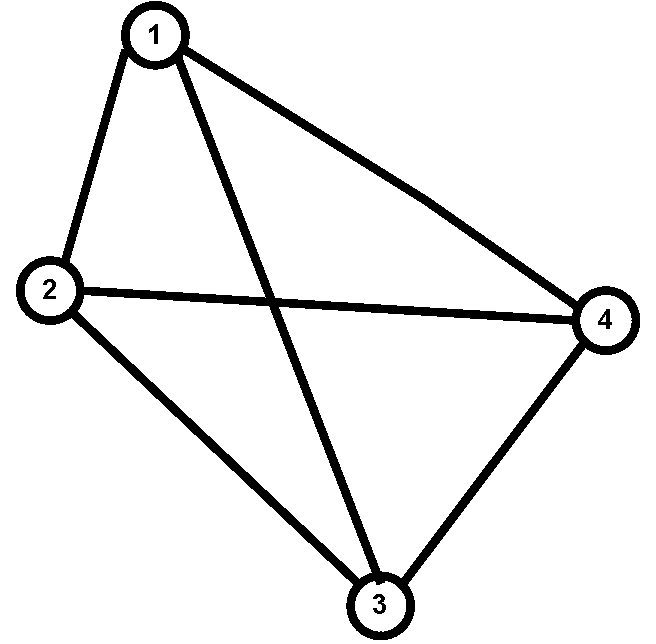
\includegraphics[width=.25\textwidth]{whole_graph.pdf} }}%
    \qquad
    \subfloat[\centering $S_0$]{{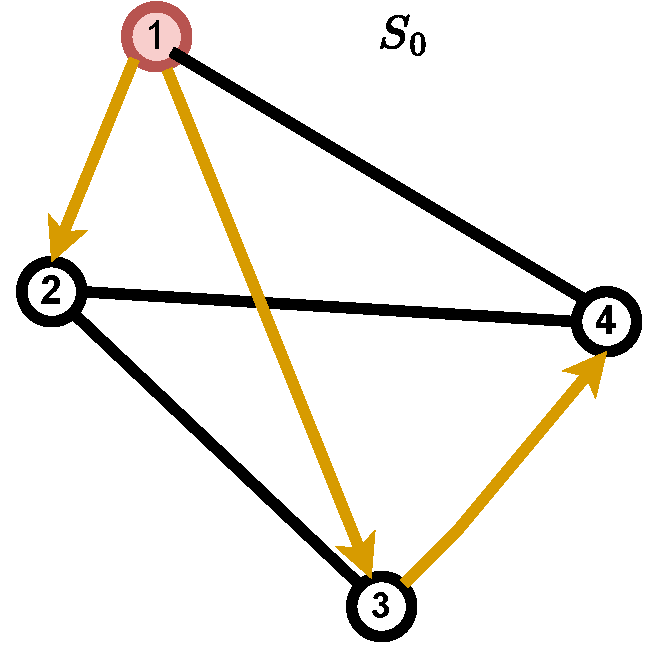
\includegraphics[width=.25\textwidth]{graph_0.pdf} }}%
    \qquad
    \subfloat[\centering $S_3$]{{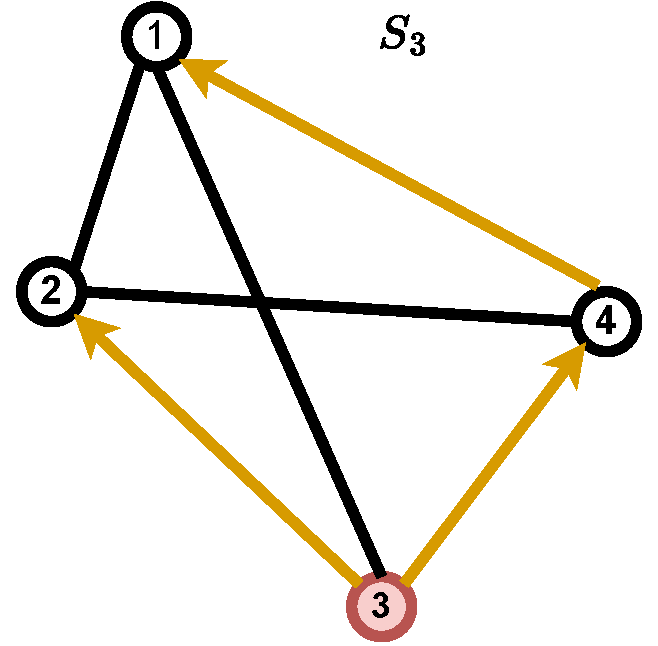
\includegraphics[width=.25\textwidth]{graph_3.pdf} }}%
    \caption{An example of an arborescene chain. The table above is a random walk over graph $G$. Then by Definition \ref{def:forward}, $S_0 = \{[1, 2], [1, 3], [3, 4]\}$ and $S_3 = \{[3, 4], [4,1], [3,2] \}$}%
    \label{fig:example-forward}%
\end{figure}


\begin{proposition}
   $(S_j; -\infty < j < \infty)$ is an irreducible and reversible Markov chain. 
\end{proposition}

\begin{proof}
Irreducibility and reversibility are directly from the assumption that $G$ is connected and unweighted. 
\end{proof}


\begin{theorem}
    Let $N(G)$ be the number of spanning trees $t$ of $G$. Then
$P(T = t) = 1/N(G)$ for each $t$ produced by Algorithm 1.
\end{theorem} 

We will first prove a simpler case when the graph is r-regular. 


\begin{proof}
    Let $G$ be an r-regular graph. Let $(X_j; -\infty < j < \infty)$ and $(S_j; -\infty < j < \infty)$ be the Markov chain of the nodes and arborescences introduced previously. 

Consider the transition matrix $Q$ for $S_j$ in reversed time:
$$Q(t, t') = P(S_{-1} = t' | S_0 = t)$$

Then
\begin{itemize}
    \item Given $t$, there are exactly $r$ trees $t'$ such that $Q(t, t') = \frac{1}{r}$ and $Q(t, t') = 0$ for other trees. 
    \item Given $t'$, there are exactly $r$ trees $t$ such that $Q(t, t') = \frac{1}{r}$ and $Q(t, t') = 0$ for other trees. 
\end{itemize}

This is because $X_{-1}$ has $\frac{1}{r}$ probability to be each of the $r$ neighbours of $v$. Each possibility leads to $S_{-1}$ being some tree $t'$, and these also are the only possibilities. A similar argument can be made going from $S_{-1}$ to $S_0$. Therefore, $Q$ is doubly-stochastic, which further implies that the stationary distribution of $S_j$ is uniform. 
\end{proof}

To extend the above proof to non-regular graphs, we first make the observation that each tree $t$ has $r(v)$ neighbours, where $v$ is the root of the tree. This implies that we can swap $r$ in the two bullet points above with the degree of the roots. It then follows that the stationary distribution of $t$ is proportional to the degree of its root. Thus, all directed spanning trees rooted at the same node are uniform. Since our trees are undirected and unrooted, all $T$ in Algorithm 1 are uniform. 
\section{Faster Generation of Spanning Trees}

In this section, we will introduce a faster algorithm for generating \emph{approximately uniform} random spanning trees. In particular, we focus on the generation of $\delta-$random spanning trees:

\begin{definition}[$\delta-$random spanning trees]
A randomized algorithm $A$ that generates $\delta-$random spanning trees outputs a random spanning tree $T$ with probability $p(T)$ that is \emph{$\delta-$far from uniform}, i.e., 
$$\frac{1-\delta}{|\mathcal{T}(G)|}\leq p(T) \leq \frac{1+\delta}{|\mathcal{T}(G)|}$$
where $\mathcal{T}(G)$ is the set of spanning trees of $G$.
\end{definition}

% \subsection{$\delta-$random spanning trees and arborescences}

% \subsection{Algorithm}

With the same reasoning as before, if we get a procedure that generates $\delta-$random arborescences, it also gives a procedure that generates $\delta-$random spanning trees. 

\cite{kelner2009faster} introduces a faster generation algorithm which generates $\delta-$random spanning trees in expected time of $\bigotilde(m\sqrt{n}\log(1/\delta))$. For brevity of illustration, we will focus on a simplified algorithm that gives an expected running time of $\bigotilde(m^2/\sqrt{n}\log(1/\delta))$, which shares the same spirit.

%Haonan: Moved to part 1
%Before discussing the algorithm, it will be useful to introduce \emph{arborescences} defined as below:
%\begin{definition}{Arborescence}    
%    For a given $s \in G$, an arborescence $T$ \emph{rooted at $s$} is a directed spanning tree of $G$ where all vertices in $G \setminus \set{s}$ have \emph{exactly one} incoming arc.
%\end{definition}

%It is easy to check that there is a one-to-one correspondence between spanning trees of $G$ and arborescences rooted at $s$: given any spanning tree, there is a unique way of directing its edges to make it an arborescence rooted at $s$; conversely, given any arborescence rooted at $s$, one can obtain a spanning tree by simply disregarding the direction of the edges.
%Therefore, if we get a procedure that generates ($\delta-$random) arborescences, it also gives a procedure that generates ($\delta-$random) spanning trees. 
%In fact, the random walk algorithm simulates the generation of arborescences.

The key idea of the algorithm is the observation that the random walk algorithm may spend a long time walking in regions that have already been covered. Indeed, the random walk algorithm has a running time of $O(mn)$, while only a tiny fraction $O(n)$ is used for recovering an arborescence.
Therefore, the algorithm seeks to obtain a shortcut that cuts out the random walk corresponding to visiting already explored parts of $G$.
The essential steps are to first decompose the graph into small subgraphs that can be quickly covered, and then shortcut the walk inside each subgraph \emph{if it is already covered}.

\subsection{Decompose the graph}
First, we define the $(\phi, \gamma)$-Decomposition that will permit the implementation of the fast generation algorithm. 
Let $(D_1, \dots, D_k, S, C)$ denote a partition of $G$, where $D_i$ are disjoint subgraphs, $S=V(G) \setminus \bigcup_i V(D_i)$ is the set of remaining vertices, and $C=E(G) \setminus \bigcup_i E(D_i)$ is the set of edges not entirely contained inside one of $D_i$. 
For a given $D_i$, let $C(D_i)$ be the subset of $C$ incident to $D_i$ and $U(D_i)$ be the set of vertices of $D_i$ incident to an edge from $C$.

\begin{definition}[$(\phi, \gamma)$-decomposition]
   $(D_1, \dots, D_k, S, C)$ is a $(\phi, \gamma)$-decomposition if:
   \label{def:decomposition}
\begin{enumerate}
    \item $|C| \leq \phi |E(G)|$
    \item $\forall i$, the diameter $\gamma(D_i) \leq \gamma$
    \item $\forall i$, $|C(D_i)| \leq |E(D_i)|$
\end{enumerate}
\end{definition}
Note that the first condition ensures that the subgraphs $D_1, \dots, D_k$ contain most (all but a $\phi$ fraction of) edges in $G$.
Intuitively, the second condition ensures that each subgraph could be covered relatively quickly, using the fact that the cover time of an unweighted graph $G'$ with diameter $\gamma(G')$ is at most $O(|E(G')|\gamma(G'))$ \cite{aleliunas1979random}.

For reasons that will become clear later, we consider a specific decomposition that can be quickly computed, shown by the following lemma:
\begin{lemma}[Obtaining good ($(\phi, \gamma)$-decompositions]
\label{lem:decompose}
For $G$ and any $\phi=o(1)$, a $(\phi, \bigotilde(1/\phi))$-decomposition of $G$ can be computed in time $\bigotilde(m)$.
\end{lemma}
We omit the proof for brevity and refer interested readers to Lemma 13 and its proof in \cite{kelner2009faster}.

\subsection{Decompose the walk}
Then, we considet the random walk $X=(X_i)$  over the decomposed graph started from a vertex chosen by the stationary distribution $G$. 
Let $\tau$ be the cover time of $G$, i.e., the first time that the walk visits all the vertices of $G$.
The result in \cite{aleliunas1979random} yields that $E[\tau]=O(mn)$ which is the expected time of traditional random walk.

We decompose the walk over decomposed $G$.
Let $Z$ and $Z_i$ be the random variables corresponding to the number of times that $X$ traverses edges from $C$ and inside $D_i$ respectively. 
By definition, we have that $\tau=\sum_i Z_i + Z$. The following lemma establishes the expectation of $Z$:
\begin{fact}
    \label{fact:traverse}
    The expected traversed time in $C$ is $E(Z)=O(\phi mn)$. 
\end{fact}
\begin{proof}
    Since the random walk starts from the stationary distribution of $G$, the expected number of traversals of edges from $C$ is just proportional to its size. Therefore, the assumption $|C| \leq \phi |E(G)|$ implies the above fact.
\end{proof}

As discussed before, we will be interested in the cover time for each subgraph. In particular, let $Z^*_i$ be the random variable corresponding to the number of traversals inside $D_i$ until $X$ explores the whole subgraph $D_i$, we have that:
\begin{lemma}[Expected cover time for subgraphs]
    \label{lem:cover}
    $E[Z_i^*] = \bigotilde(|E(D_i)|\gamma(D_i))$.
\end{lemma}
\begin{proof}
Let us fix $D = D_i$. For a vertex $v \in V(D)$, let $d_G(v)$ be the degree of $v$ in $G$ and $d_D(v)$ be the degree of $v$ in $G$. For $u,v \in U(D)$, let $p_{u,v}^D$ be the probability that a random walk in $G$ that starts at $u$ will reach $v$ through a path that does not pass through any edge inside $D$. Consider a (weighted) graph $D'$, which we obtain from $D$ by adding, for each $u,v \in U(D)$, an edge $(u, v)$ with weight $d_G(u) p_{u,v}^D$. We note that if we take our walk $X$ and filter out of the vertices that are not from $D$, then the resulting "filtered" walk $Y_D$ will just be a natural random walk in $D'$. As a result, it is easy to see that, in this case, $E[Z_i^*]$ can be upper-bounded by the expected time needed by a random walk in $D'$, started at arbitrary vertex, to visit all of the vertices in $D'$ and then reach some vertex in $U(D)$. Therefore, to bound $E[Z_i^*]$, it suffices to bound the cover time of $D'$. The cover time of undirected graph $G'$ is at most $2\log|V(G')|H_{max}(G')$, where $H_{max}(G')$ is the maximal hitting time. Following the results of \cite{aleliunas1979random}, we have $H_{max}(G') \leq |E(G')|\gamma(G')$. 
\end{proof}
%\begin{proof}
    %\textcolor{red}{TODO}: Refer to Lemma 6 in \cite{kelner2009faster}.
%\end{proof}

\subsection{Shortcut the walk}
Recall that the key idea of the algorithm is to shortcut the trajectory inside $D_i$ after $D_i$ has already been covered. 
More specifically, consider the walk after $D_i$ is covered, this means that we already know for all edges $v \in V(D_i)$ which arc $e_v$ should be added to the arborescence. 
Any further walk inside $D_i$ provides no new information for constructing the arborescence, and could be shortcutted.

\begin{figure}[t!]
        \centering
        \begin{subfigure}[b]{.35\textwidth}
            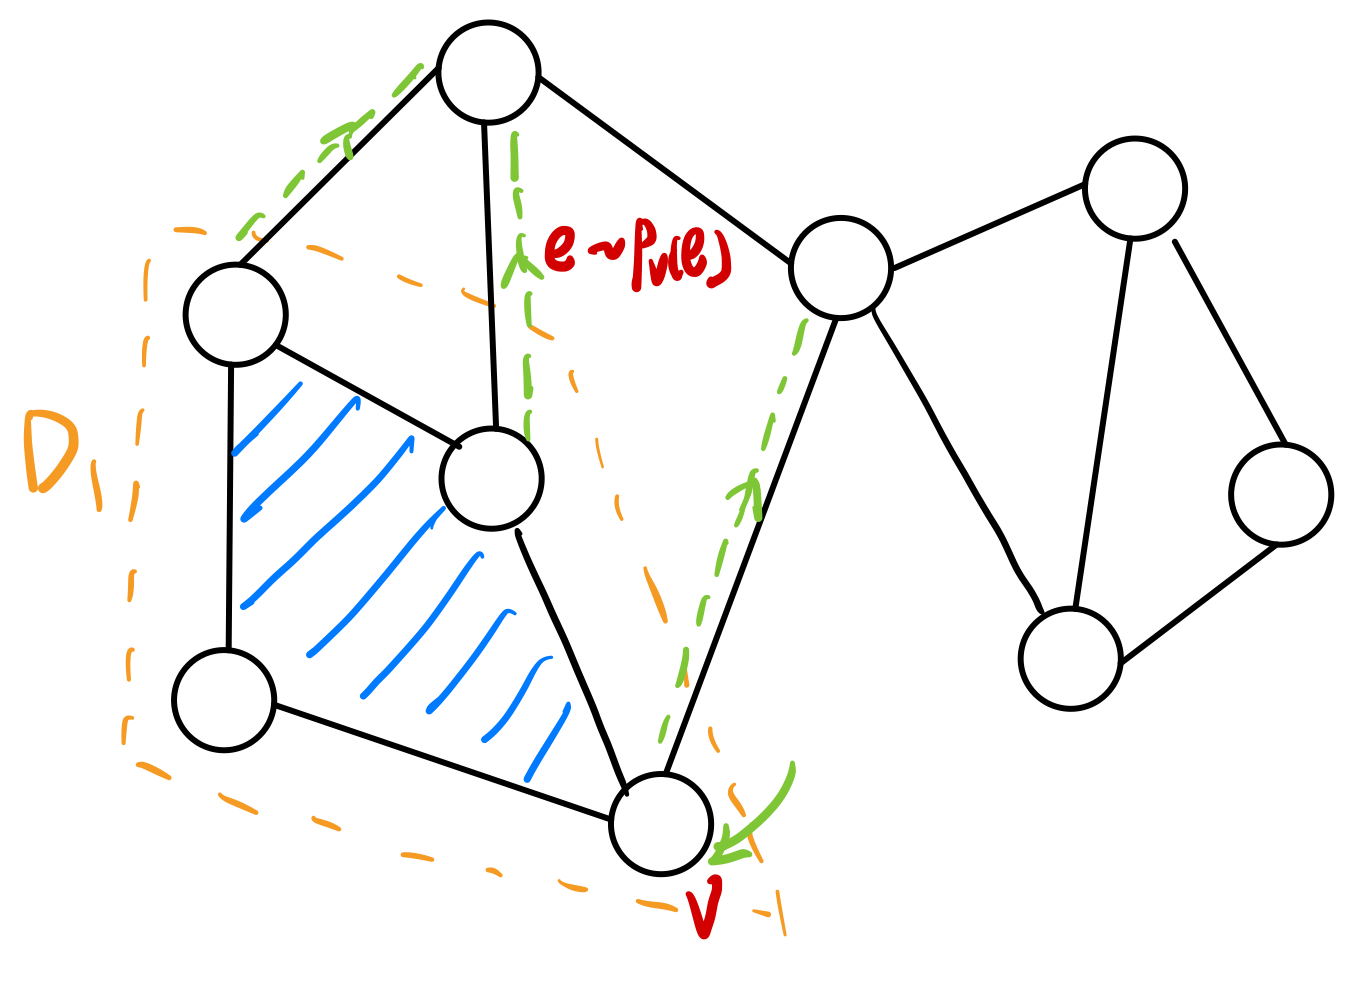
\includegraphics[width=0.9\linewidth, trim={1cm 1cm 1cm 0},clip]{figs/shortcut_impl.jpeg}
            \caption{}
            \label{fig:shortcut_impl}
        \end{subfigure}
        \begin{subfigure}[b]{.62\textwidth}
            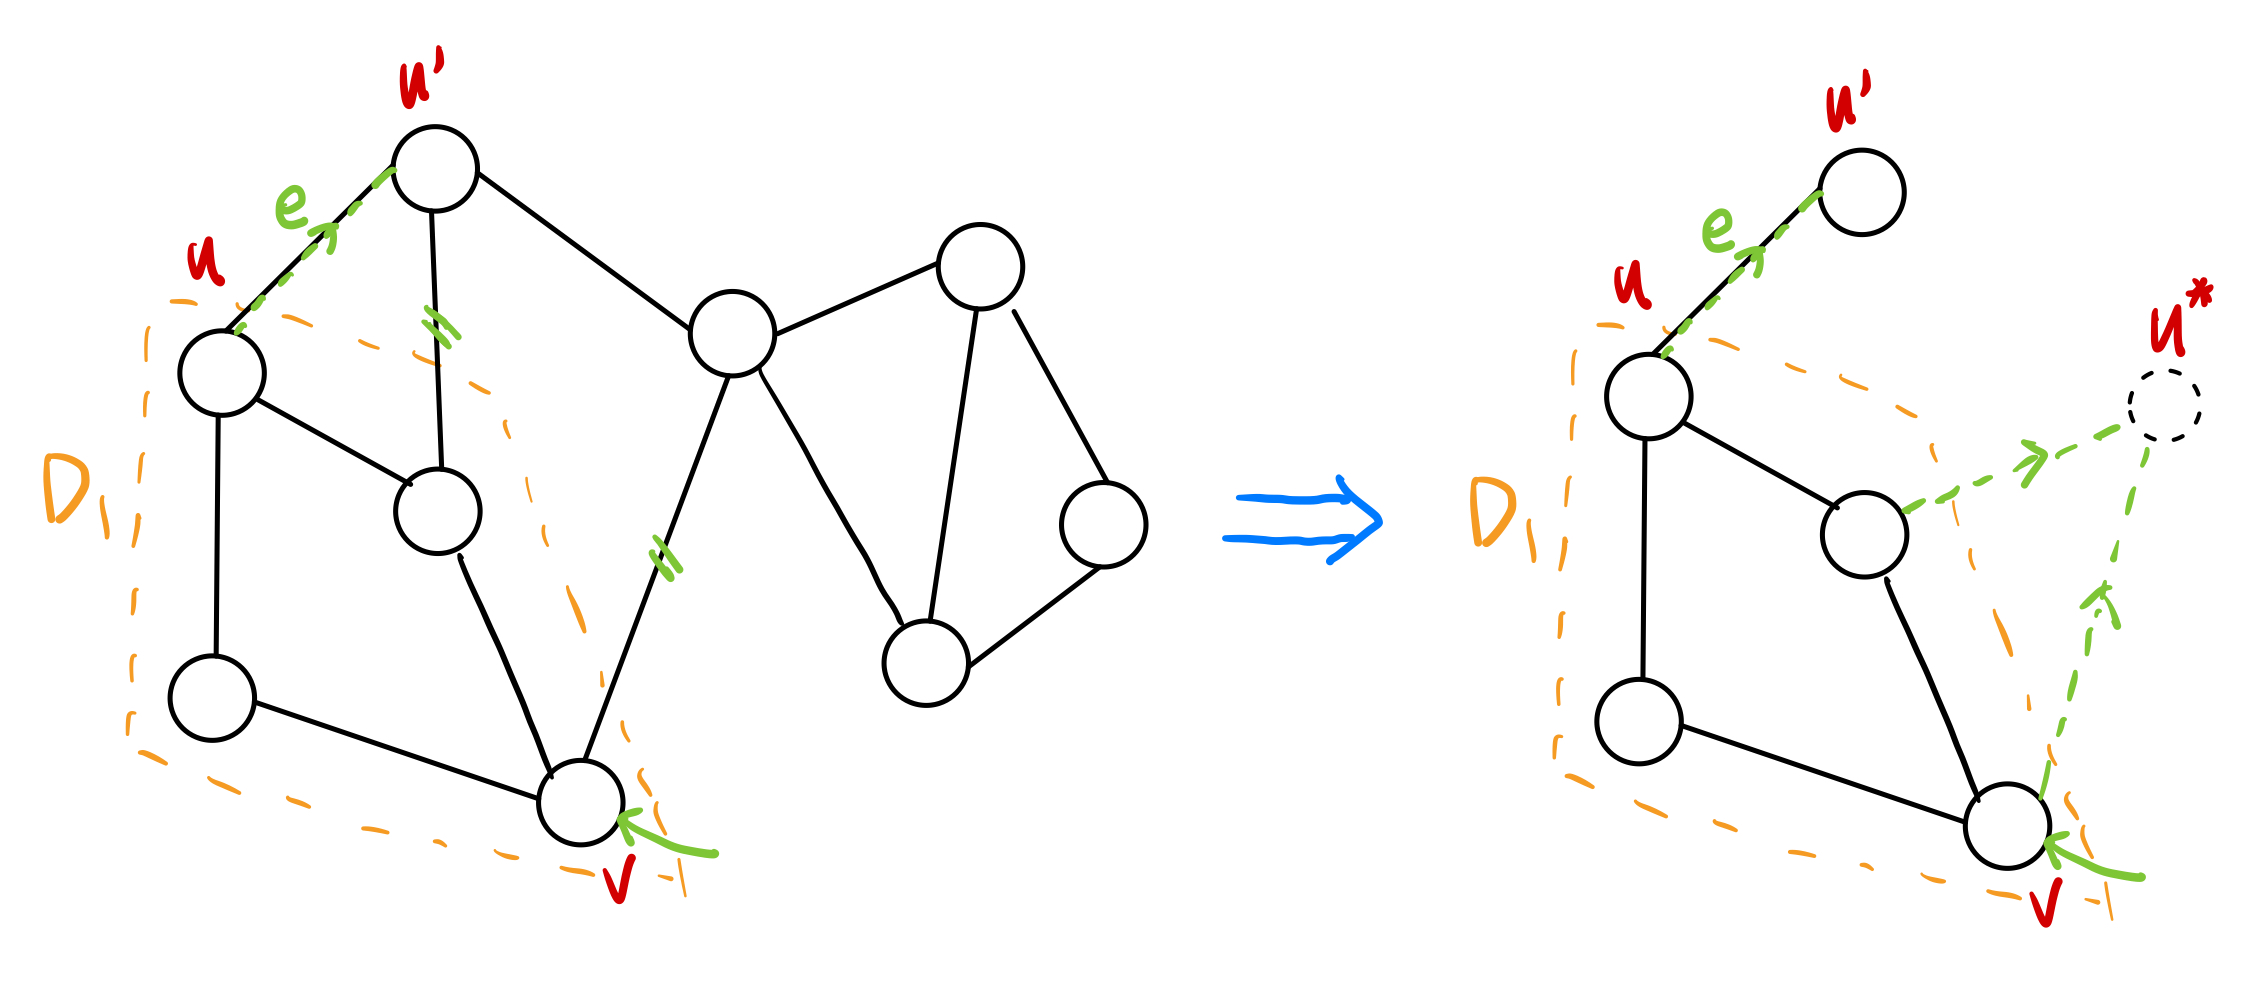
\includegraphics[width=0.95\linewidth, trim={1cm 1cm 1cm 0},clip]{figs/compute_prob.jpeg}
            \caption{}
            \label{fig:compute_prob}
        \end{subfigure}
        \caption{(a) The shortcut of trajectory inside $D_1$ Is implemented by $P_v(e)$ that characterizes the probability of $X$ leaving $D_1$ through edge $e$ after entering through vertex $v$; (b) The illustration for computing $P_v(e)$ by adding a dummy node $u^*$ which connects to all other leaving edges.}
\end{figure}

The main tool for implementing the shortcut is $P_v(e)$ that characterizes the probability of $X$ leaving $D_i$ \emph{through edge $e$ after entering through vertex $v$}, see Fig.\ \ref{fig:shortcut_impl} for an illustration.
If we know $P_v(e)$ for all $v \in V(D_i)$ and all $e \in C(D_i)$, then we could essentially immediately choose the leaving edge $e$ upon entering $v$ without computing the explicit trajectory in $D_i$.

To formalize the intuition, let $\bar{X}=(\Bar{X}_1, \dots, \Bar{X}_m)$ be a decomposition of the walk $X=(X_1, \dots, X_\tau)$ into contiguous blocks $\Bar{X}_j$ that are contained in $D_{i_j}$ for $i_j \in \{0, \dots, k\}$, where $D_0=S$.
We construct the shortcutted walk $\Tilde{X}=(\Tilde{X}_i)$ by processing $\bar{X}$ block by block: 
if $D_{i_j}$ has not been covered or $i_j=0$, we copy $\Bar{X}_j$ to $\Tilde{X}$, otherwise we copy only the first and last entries of the block.

With $P_e(v)$, the following lemma establishes that $\Tilde{X}$ can be simulated efficiently:
\begin{lemma}[Simulating $\tilde{X}$ with $P_v(e)$]
\label{lem:simulate}
        Knowing $P_v(e)$ for all $e \in C(D_i), v \in V(D_i)$ and $i$, we can preprocess these values in $\bigotilde(\phi mn)$ time and it allows simulation of $l$ steps of $\tilde{X}$ in time $\bigotilde(l)$.
\end{lemma}
\begin{proof}
    Simulating $\Tilde{X}$ before $D_i$ is covered is straightforward. The only thing to show is that the shortcutting of blocks can be simulated efficiently. To show this, we consider some $i$ and $v \in U(D_i)$, and construct an array $A_v(m)$ where $A_v(m) = \sum_
{1\leq j \leq m} P_v(e_j)$ for $m \in \{1, \dots, |C(D_i)|\}$ in $\bigotilde(|C(D_i)|)$. So we can construct for all $v \in U(D_i)$ in $\bigotilde(|C(D_i)||V(D_i)|)$. Summing over all $D_i$ gives the above bound on preprocessing time.
Furtheremore, this array enables choosing $e$ with $P_v(e)$ with binary search in polylogarithmic time. 
\end{proof}

From this lemma, we can show that we can find a random arborescence of $G$ efficiently:
\begin{lemma}[Finding a random arborescence]
\label{lem:find_abr}
        Given a $(\phi, \gamma)$-decomposition of $G$ and $P_v(e)$, we can find a random arborescence of $G$ in expected time $\bigotilde(m(\gamma+\phi n))$.
\end{lemma}
\begin{proof}
    We only need to compute the expected length of the shortcutted walk $\Tilde{X}$, which is upper-bounded by the following quantity:
    $$\sum_i \underbrace{E[Z_i^*]}_{\text{cover time of}~D_i} + \underbrace{E[Z]}_{\text{traversals in}~C} + \underbrace{2E[Z]}_{\text{shortcutted traversals }}$$
    The first and the second terms are obvious, and the last term is due to the fact that the two vertices that remain in $\Tilde{X}$ after shortcutting some block from $X$ can be amortized into the number of traversals by $X$ of some edges in $C$.
    By the second assumption in Definition \ref{def:decomposition}, Fact \ref{fact:traverse}, Lemma \ref{lem:cover}, we get that $\sum_i E[Z_i^*] + 3 E[Z] =\bigotilde(\sum_i |E(D_i)\gamma + \phi mn|) = \bigotilde(m(\gamma + \phi n))$. By Lemma \ref{lem:simulate}, the shortcutted work can be simulated in expected time $\bigotilde(m(\gamma + \phi n))$.
\end{proof}

Then the remaining question is whether we can compute $P_e(v)$ efficiently, established by the following lemma:
\begin{lemma}[Computing $P_v(e)$]
    \label{lem:compute_prob}
    Given a $(\phi, \gamma)$-decomposition of $G$, we can compute multiplicative $(1+\varepsilon)$-approximations of $P_v(e)$ in time $\bigotilde(\phi m^2 \log(1/\varepsilon))$
\end{lemma}
\begin{proof}
    Let us fix some $D=D_i$ and an edge $e=(u, u') \in C(D)$ with $u \in U(D)$. Consider a graph $D'$ obtained by adding a dummy node $u^*$ to $D$ and then connecting all other leaving edges to $u^*$, i.e., for each $(w, w') \in C(D) \setminus \{e\}$, we add an edge $(w, u^*)$ (note that $w'$ can be equal to $u'$), see Fig. \ref{fig:compute_prob} for an illustration. Note that $P_v(e)$ is the probability that the walk started at $v$ will \emph{hit $u'$ before $u^*$}, which can be quickly computed using \emph{electrical flows}.

    In particular (see, e.g., \cite{lovasz1993random}), we can treat $D'$ as an electrical circuit where we impose voltage of $1$ at $u'$ and $0$ at $u^*$, then the voltage achieved at $v$ is exactly equal to $P_v(e)$. We can compute a $(1+\varepsilon)$-approximation in $\bigotilde(|E(D')|\log1/\varepsilon)$ using the linear solver in \cite{spielman2014nearly}. Computing for each $e \in C(D)$ and store the probabilities for all vertices $v$, the total running time can be bounded by $\bigotilde(|C|\sum_i |E(D_i)| \log 1/\varepsilon)=\bigotilde(\phi m^2 \log 1/\varepsilon)$, where we use the fact that $|E(D')| = |E(D)| + |C(D)| \leq 2 |E(D)|$ by assumption 3 in Definition \ref{def:decomposition}.
\end{proof}

Note that the above lemma only gives an approximation of $P_v(e)$. We need to show that it is sufficient for controlling the overall error and maintaining a good running time:
\begin{lemma}[An approximate $P_v(e)$ is sufficient]
    \label{lem:sufficiency}
    Given a $(\phi, \gamma)$-decomposition of $G$ and multiplicative $(1+\varepsilon)$-approximation of $P_v(e)$, we can generate a $\delta-$random arborescence of $G$ in expected time $\bigotilde(m^2(\gamma+\phi n))$ as long as $\varepsilon \leq \delta / mn$.
\end{lemma}
%\begin{proof}
We omit the proof for brevity and refer interested readers to Lemma 10 and its proof in \cite{kelner2009faster}.%\cite{kelner2009faster}.    
%\end{proof}


Putting all together, we have the theorem establishing the running time of the algorithm:
\begin{theorem}[Total complexity]
    For any $\delta>0$, we can generation a $\delta-$random spanning tree of $G$ in expected time of $\bigotilde(m/\sqrt{n}\log(1/\delta))$.
\end{theorem}
\begin{proof}
    Let $\phi=1/n^{1/2}, \varepsilon=\delta/mn$, the total expected time can be decomposed as:
    \begin{enumerate}
        \item Get a $(1/n^{1/2}, \bigotilde(n^{1/2}))$-decomposition: $\bigotilde(m)$ (Lemma \ref{lem:decompose}).
        \item Compute estimate of $P_v(e)$: $\bigotilde(m^2/\sqrt{n}\log(1/\delta))$ (Lemma \ref{lem:compute_prob}).
        \item Generate a $\delta$-arborescence: $\bigotilde(m\sqrt{n})$ (Lemma \ref{lem:find_abr}, Lemma \ref{lem:sufficiency}).
    \end{enumerate}
    Summinga all together, we have the total running time of $ \bigotilde(m^2/\sqrt{n}\log(1/\delta))$.
\end{proof}

We refer interested readers to Sec. 4 in \cite{kelner2009faster} for an improved algorithm with $\bigotilde(m\sqrt{n}\log(1/\delta))$, which is obtained by a stronger decomposition and a slightly different random walk.



% \bibliography{ref}
% \bibliographystyle{plain}
% \bibliographystyle{abbrv}%

\printbibliography
\end{document}